\documentclass[11pt,a4paper,titlepage,oneside]{article}

% --- Paquets de base ---
\usepackage[utf8]{inputenc}
\usepackage[T1]{fontenc}
\usepackage[french]{babel}
\usepackage[top=1.5cm, bottom=5cm, hmargin=3cm]{geometry}
\usepackage{graphicx}
\usepackage{listings}
\usepackage{array, pdfpages}
\usepackage[breaklinks]{hyperref}
\usepackage{tabularx}
\usepackage{makecell}
\usepackage{float}
\usepackage{titlesec}
\usepackage[export]{adjustbox}
% --- Bibliographie ---
\usepackage[
style=numeric,
sorting=ynt
]{biblatex}

\addbibresource{biblio.bib}
% --- Mise en page (Header/Footer) ---
\usepackage{fancyhdr}
\pagestyle{fancy}
\fancyhf{} 
\rhead{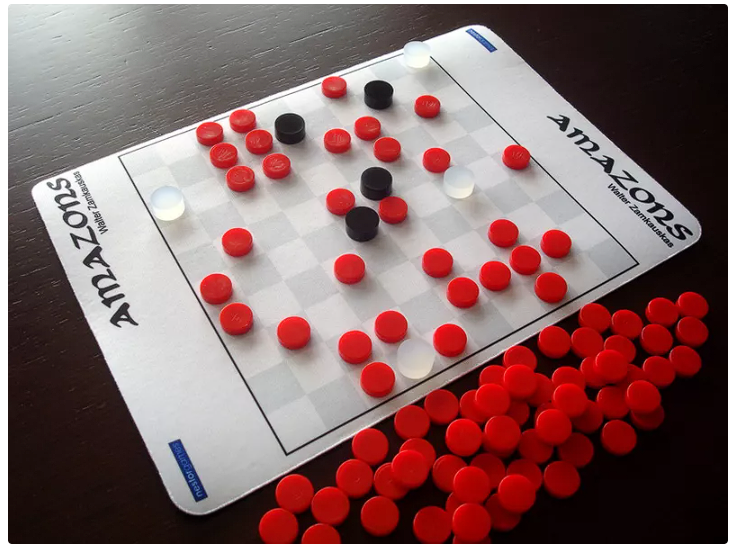
\includegraphics[width=2cm]{Amazones}} 
\cfoot{\thepage} 
\headheight = 1,5cm
\headsep = 0.75cm
% --- Personnalisation des titres ---
\usepackage{titlesec}
\titleformat{\section}[display]
  {\normalfont\huge\bfseries}
  {}
  {0pt}
  {\huge}

\renewcommand{\thepart}{\arabic{part}}
\begin{document}

    % --- Page de garde ---
    \begin{titlepage}
        \fontfamily{pag}\selectfont
        \begin{center}\normalsize
            \MakeUppercase{Informatique M1 \hfill Groupe Amazone - C \hfill 2025-2026}
        \end{center}
        \vspace*{0.1cm}
        \hrule
        \vspace*{0.2cm}
        \vspace*{2cm}
        \begin{center}\Huge
            \textsc{\textbf{Rapport Projet M1}}
        \end{center}
        \hrule
        \begin{center}
            \MakeUppercase{Rapport effectué dans le cadre du projet de semestre 8}
        \end{center}
        \vspace*{2cm}
        \begin{center}\Large
            Nicolas \textsc{Caminade}\\ \vspace{0.3cm}
            Tanguy \textsc{Decabrat}\\ \vspace{0.3cm}
            Anya \textsc{Bazizi}\\ \vspace{0.3cm}
            Younes \textsc{Ouaammou}\\ \vspace{0.3cm}
            Thomas-Alexandre \textsc{Moreau}
        \end{center}
        \vfill
        \begin{center}\normalsize
            \MakeUppercase{Rapport Projet --- Semestre 8}
        \end{center}
    \end{titlepage}

    % --- Sommaire ---
    \newpage
    \renewcommand{\contentsname}{Sommaire}
    \setcounter{tocdepth}{3} 
    \tableofcontents

    
    
\newpage
    \section{Présentation du projet}
\subsection{Historique des Amazones}

Le jeu des Amazones, créé en 1988 par l'Argentin Walter Zamkauskas, est un défi majeur pour l'informatique, dont l'histoire est la suivante :
\begin{itemize}
    \item En 2005, l'équipe de Furtak prouve mathématiquement que résoudre ce jeu est PSPACE-complet, une classe de difficulté bien supérieure à celle des problèmes NP standards. \cite{furtak2005generalized}
    \item Richard Lorentz, avec son programme Invader, démontre ensuite que l'approche statistique du Monte Carlo Tree Search (MCTS) est la seule viable face à l'explosion combinatoire du jeu en 2017.\cite{lorentz2008amazons}
    \item Depuis lors, des chercheurs intègrent désormais le Deep Learning et les réseaux de neurones pour tenter de surpasser cet algorithme.\cite{9534274}
    
    
\end{itemize}

    \subsection{Règles}

    Le Jeu des Amazones se pratique sur un damier, traditionnellement de $10 \times 10$ cases. Chaque joueur possède quatre amazones, placées dans une configuration initiale spécifique qui définit le point de départ .
    
    \paragraph{Objectif du jeu :}Le but est de complètement bloquer les mouvements de l'adversaire en occupant ou en bloquant stratégiquement l'espace. La victoire est acquise lorsqu'un joueur parvient à bloquer toutes les amazones adverses, ne lui laissant plus aucune possibilité de mouvement.
     
    \paragraph{Déroulement d'un tour :}Chaque action d'un joueur est impérativement composée de deux phases successives :
    \begin{enumerate}
    
    \item \textbf{Le déplacement :} Le joueur choisit l'une de ses amazones et la déplace en ligne droite (verticalement, horizontalement ou en diagonale) vers une case libre. Le mouvement est identique à celui de la dame aux échecs, mais l'amazone ne peut ni traverser ni s'arrêter sur une case occupée par une autre pièce ou une flèche.
    \item \textbf{Le tir de flèche :} Après son déplacement, cette même amazone doit tirer une flèche depuis sa nouvelle position. La flèche suit les mêmes règles de trajectoire qu'une amazone. La case d'arrivée de la flèche est alors marquée d'un blocage définitif pour le reste de la partie.
    \end{enumerate}
    \paragraph{Fin de partie et variantes}Contrairement à d'autres jeux de plateau, le Jeu des Amazones ne connaît pas de situation de match nul par répétition ou par épuisement de matériel. Puisque chaque tour réduit irrémédiablement le nombre de cases disponibles, le jeu se termine forcément par le blocage complet d'un joueur. Bien que le format $10 \times 10$ soit le standard, il existe des variantes ($6 \times 6$ ou $8 \times 8$) avec un nombre d'amazones adapté, permettant des parties plus rapides tout en conservant la complexité tactique du jeu.

    \begin{figure}[ht]
    \centering
    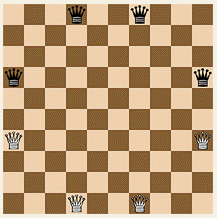
\includegraphics[width=0.22\textwidth]{defaultStateboard.png} 
    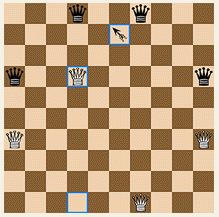
\includegraphics[width=0.22\textwidth]{1wallplacedboard.png}
    \caption{Évolution d'une partie : position initiale et premier coup \cite{img0} \cite{img1}}
\end{figure}

    \subsection{Complexité} \label{sec:complexite}
        Le jeu des Amazones est un jeu d'une très grande complexité \cite{Complexite}.

\begin{table}[H]
    \centering
\renewcommand{\arraystretch}{1.5}
\resizebox{\textwidth}{!}{
\begin{tabular}{ | p{4.5cm} || c | c | c | }
    \hline
    % --- Première Ligne (En-têtes) ---
    \textbf{} & \textbf{Échecs} & \textbf{Amazones} & \textbf{Go} \\
    \hline

    % --- Reste du tableau ---
    Facteur Branch. Initial
    & $\mathtt{\sim}$ 20
    & \makecell{$\mathtt{\sim}$ 2176}
    & $\mathtt{\sim}$ 361 \\
    \hline
    Facteur Branch. Moyen
    & $\mathtt{\sim}$ 35
    & \makecell{$\mathtt{\sim}$ 374 joueur de départ \\ $\mathtt{\sim}$ 299 deuxième joueur \\ $\mathtt{\sim}$50 durant la fin de partie}
    & $\mathtt{\sim}$ 250 \\
    \hline
    Nombre de tours moyen
    & $\mathtt{\sim}$ 80 
    & $\mathtt{\sim}$ 84 
    & $\mathtt{\sim}$ 150 \\
    \hline
    Cmplx. Arbre de jeu 
    & $\mathtt{\sim} 10^{123}$ 
    & $\mathtt{\sim}$ 1.09 * $10^{212}$ 
    & $\mathtt{\sim} 10^{360}$ \\
    \hline
    Cmplx. Espaces d'états
    & \makecell{de $\mathtt{\sim}$ 3.7 * $10^{43}$ à $\mathtt{\sim}$ $10^{52}$}
    & $\mathtt{\sim}$ 6.45* $10^{40}$
    & $\mathtt{\sim}$ $10^{170}$ \\
    \hline
    
\end{tabular}
}
\caption{Comparaison des complexités \cite{complexities} \cite{gocomplexity}}
\end{table}
\renewcommand{\arraystretch}{1}
        
        Comme l'illustre le tableau comparatif, la complexité des Amazones réside dans son facteur de branchement initial extrême, surpassant largement celui des échecs et du Go. Bien que la profondeur de jeu soit modérée, cette "largeur" excessive génère un arbre de jeu colossal (10$^{212}$), empêchant une exploration exhaustive de l'arbre en raison de l'explosion combinatoire des possibilités de jeu. Pour ces raisons, algorithmiquement, le défi se rapproche ainsi davantage de la résolution du Go que des échecs.
        
        Pour contourner cette explosion combinatoire, les approches modernes s'appuient sur la sélectivité : soit par des solveurs de preuve comme \textit{df-pn} \cite{dfpn}, soit par des algorithmes de jeu utilisant du \textit{Forward Pruning} \cite{fpruning} ou d'autres méthodes statistiques que nous mettons en place dans nos IA, comme dans \textit{MCTS} via l'\textit{Upper Confidence bounds applied to Trees} (UCT) \cite{uct} ou encore le \textit{Machine Learning} (ML).

    \section{Structures et algorithmes}
    \subsection{Structures de données} 
    \subsubsection{Réseaux}
    
         Pour ce qui est de la partie réseaux du projet, on utilise plusieurs structures afin de pouvoir interagir adéquatement entre les clients et le serveur.
\begin{itemize}
        \item Au niveau du serveur, on utilise un tableau de structures nommé "ConnectedClient". Ce choix a été fait par souci de simplicité et de performance. Dans ce tableau, chaque client possède un état "state" permettant d'appliquer le bon comportement au programme dans chacun des cas où il faut vérifier les états des clients ;
        
        \item Il est possible d'avoir plusieurs clients pour un même serveur. De ce fait, nous disposons d'un buffer TCP permettant de gérer la fragmentation des packets qui pourraient ne pas arriver dans de bonnes conditions ou dans le bon ordre. Par exemple, nous pourrions avoir le cas où un message arriverait en 2 morceaux. Ce tableau possède aussi, pour chaque client, leurs informations telles que leurs statistiques, noms et scores. 
        
        \item En complément de la gestion TCP, nous avons intégré une structure spécifique nommée DiscoveryContext. Celle-ci repose sur le protocole UDP en mode Broadcast. Elle agit comme une balise autonome, elle encapsule un socket UDP dédié et un timer (last broadcast time). Son rôle est de diffuser périodiquement un ping du serveur sur le réseau local sans bloquer la boucle principale. Cette architecture découplée permet aux clients d'utiliser la commande server list pour détecter les parties disponibles sans connaître l'adresse IP du serveur à l'avance, tout en isolant strictement la logique "sans connexion" (UDP) de la logique de jeu (TCP).
\end{itemize}

    \subsubsection{IA}
     \label{sec:iastruc}

    Nous connaissons déjà certaines IAs pré-requises au sein de notre architecture, et avons souhaité les optimiser au maximum afin de permettre une meilleure expérience de jeu, mais aussi une meilleure qualité des coups joués.

    De ce fait, nous avons mis en place plusieurs principes :
    \begin{itemize}
        \item L'utilisation de structures C simulant des interfaces pour réduire les dépendances et permettre le polymorphisme du code ; 
        \item Via une Factory, il est possible de générer une IA spécifique via un tableau de paramètres passé à la méthode de création, pour faciliter l'utilisation des IAs ;
        \item L'utilisation d'arbres LCRS (Left-Children Right-Sibling) (\cite{geekslcrs}) afin de réduire la charge sur la mémoire et sur le CPU pour le calcul. Le but est de réduire au plus possible la taille de la structure des millions de nœuds que nous générerons, afin d'alléger la charge CPU/MÉMOIRE et de réduire les coûts par rapport à un tableau de pointeurs classique (possiblement de taille $\mathtt{\sim}$2176, comme vu dans la section \ref{sec:complexite}, qui se verrait multiplié par la taille de la structure pour chaque nœud, d'au minimum 3 octets...).
    \end{itemize}

    \subsubsection{Moteur de Jeu}
    L'architecture des données repose intégralement sur l'utilisation de Bitboards. Le jeu des Amazones se jouant sur un plateau allant jusqu'à $11\times11$ cases, une représentation binaire nécessite 121 bits, ce qui excède la capacité des registres standards de 64 bits.

    Pour pallier à l'absence du type \texttt{uint128\_t} dans le standard C11 (et garantir la portabilité sous MSVC), nous avons conçu une structure composite personnalisée. Le plateau est segmenté en deux entiers non-signés de 64 bits :
    \begin{itemize}
        \item \texttt{low} : encode les cases d'indices 0 à 63.
        \item \texttt{high} : encode les cases d'indices 64 à 120 (les bits restants étant inutilisés).
    \end{itemize}

    La contrainte est de faire agir ces deux entiers comme une seule entité. Nous avons donc encapsulé la logique binaire dans des fonctions dédiées. 
    Si les opérateurs logiques AND, OR, XOR s'appliquent indépendamment sur chaque moitié, les décalages (SHIFT) nécessitent une propagation : les bits qui "débordent" de la partie basse sont récupérés pour être réinjectés dans la partie haute. Cette mécanique simule un type 128 bits unique, rendant la complexité interne invisible pour le reste du moteur.
    
    Cette approche permet de traiter l'ensemble du plateau en temps constant $\mathcal{O}(1)$ contre une complexité en $\mathcal{O}(N)$ en utilisant un tableau 2D. Cette optimisation permet de maximiser le nombre de nœuds explorés par l'IA.


    \subsubsection{Interface Graphique (GUI)}
    Pour l'interface graphique, nous utiliserons la bibliothèque LibGtk. Les versions 4.X offrent énormément de possibilités autant du côté de l'affichage que des interactions utilisateur, en plus d'être relativement intuitives à l'utilisation.

    Gtk utilise une application principale (GtkApplication) comme structure, ainsi qu'une fenêtre (GtkWindow) pour représenter la partie visuelle de l'application. On peut ensuite construire différents modules personnalisés (GtkWidget) comme le plateau du jeu par exemple, y ajouter des éléments dynamiques (GtkButton, GtkOverlay, ...), et également intégrer un système d'empilement de pages (GtkStack) pour fluidifier le changement de fenêtre en simulant un changement de fenêtre au lieu de recréer une nouvelle page à chaque fois.

    La structure simplifiée de l'interface du jeu serait de cette forme :
    
    \begin{description}
        \item[- GtkApplication] Cœur de l'application
        \begin{description}
            \item[- GtkWindow] Fenêtre graphique de l'application
            \begin{description}
                \item[- GtkOverlay] Module permettant de générer des alertes à l'écran, facilement modifiable à la volée. Donc le placer aussi haut dans la hiérarchie permet de ne pas en créer un par page
                \begin{description}
                    \item[- GtkStack] Gestionnaire de pages
                    \begin{description}
                        \item[- GtkWidget] Menu Principal
                        \begin{description}
                            \item[- GtkButton]
                            \item[- ...]
                        \end{description}
                        \item[- GtkWidget] Menu Singleplayer
                        \item[- ...]
                    \end{description}
                \end{description}
            \end{description}
        \end{description}
    \end{description}

    L'interface aura pour but d'être claire et simple d'utilisation, reprenant des codes visuels basiques du jeu vidéo afin de ne pas perdre l'utilisateur. Voici deux schémas afin d'illustrer ces propos :

    \begin{figure}[H]
    \centering
    \begin{minipage}{0.46\textwidth}
        \centering
        \frame{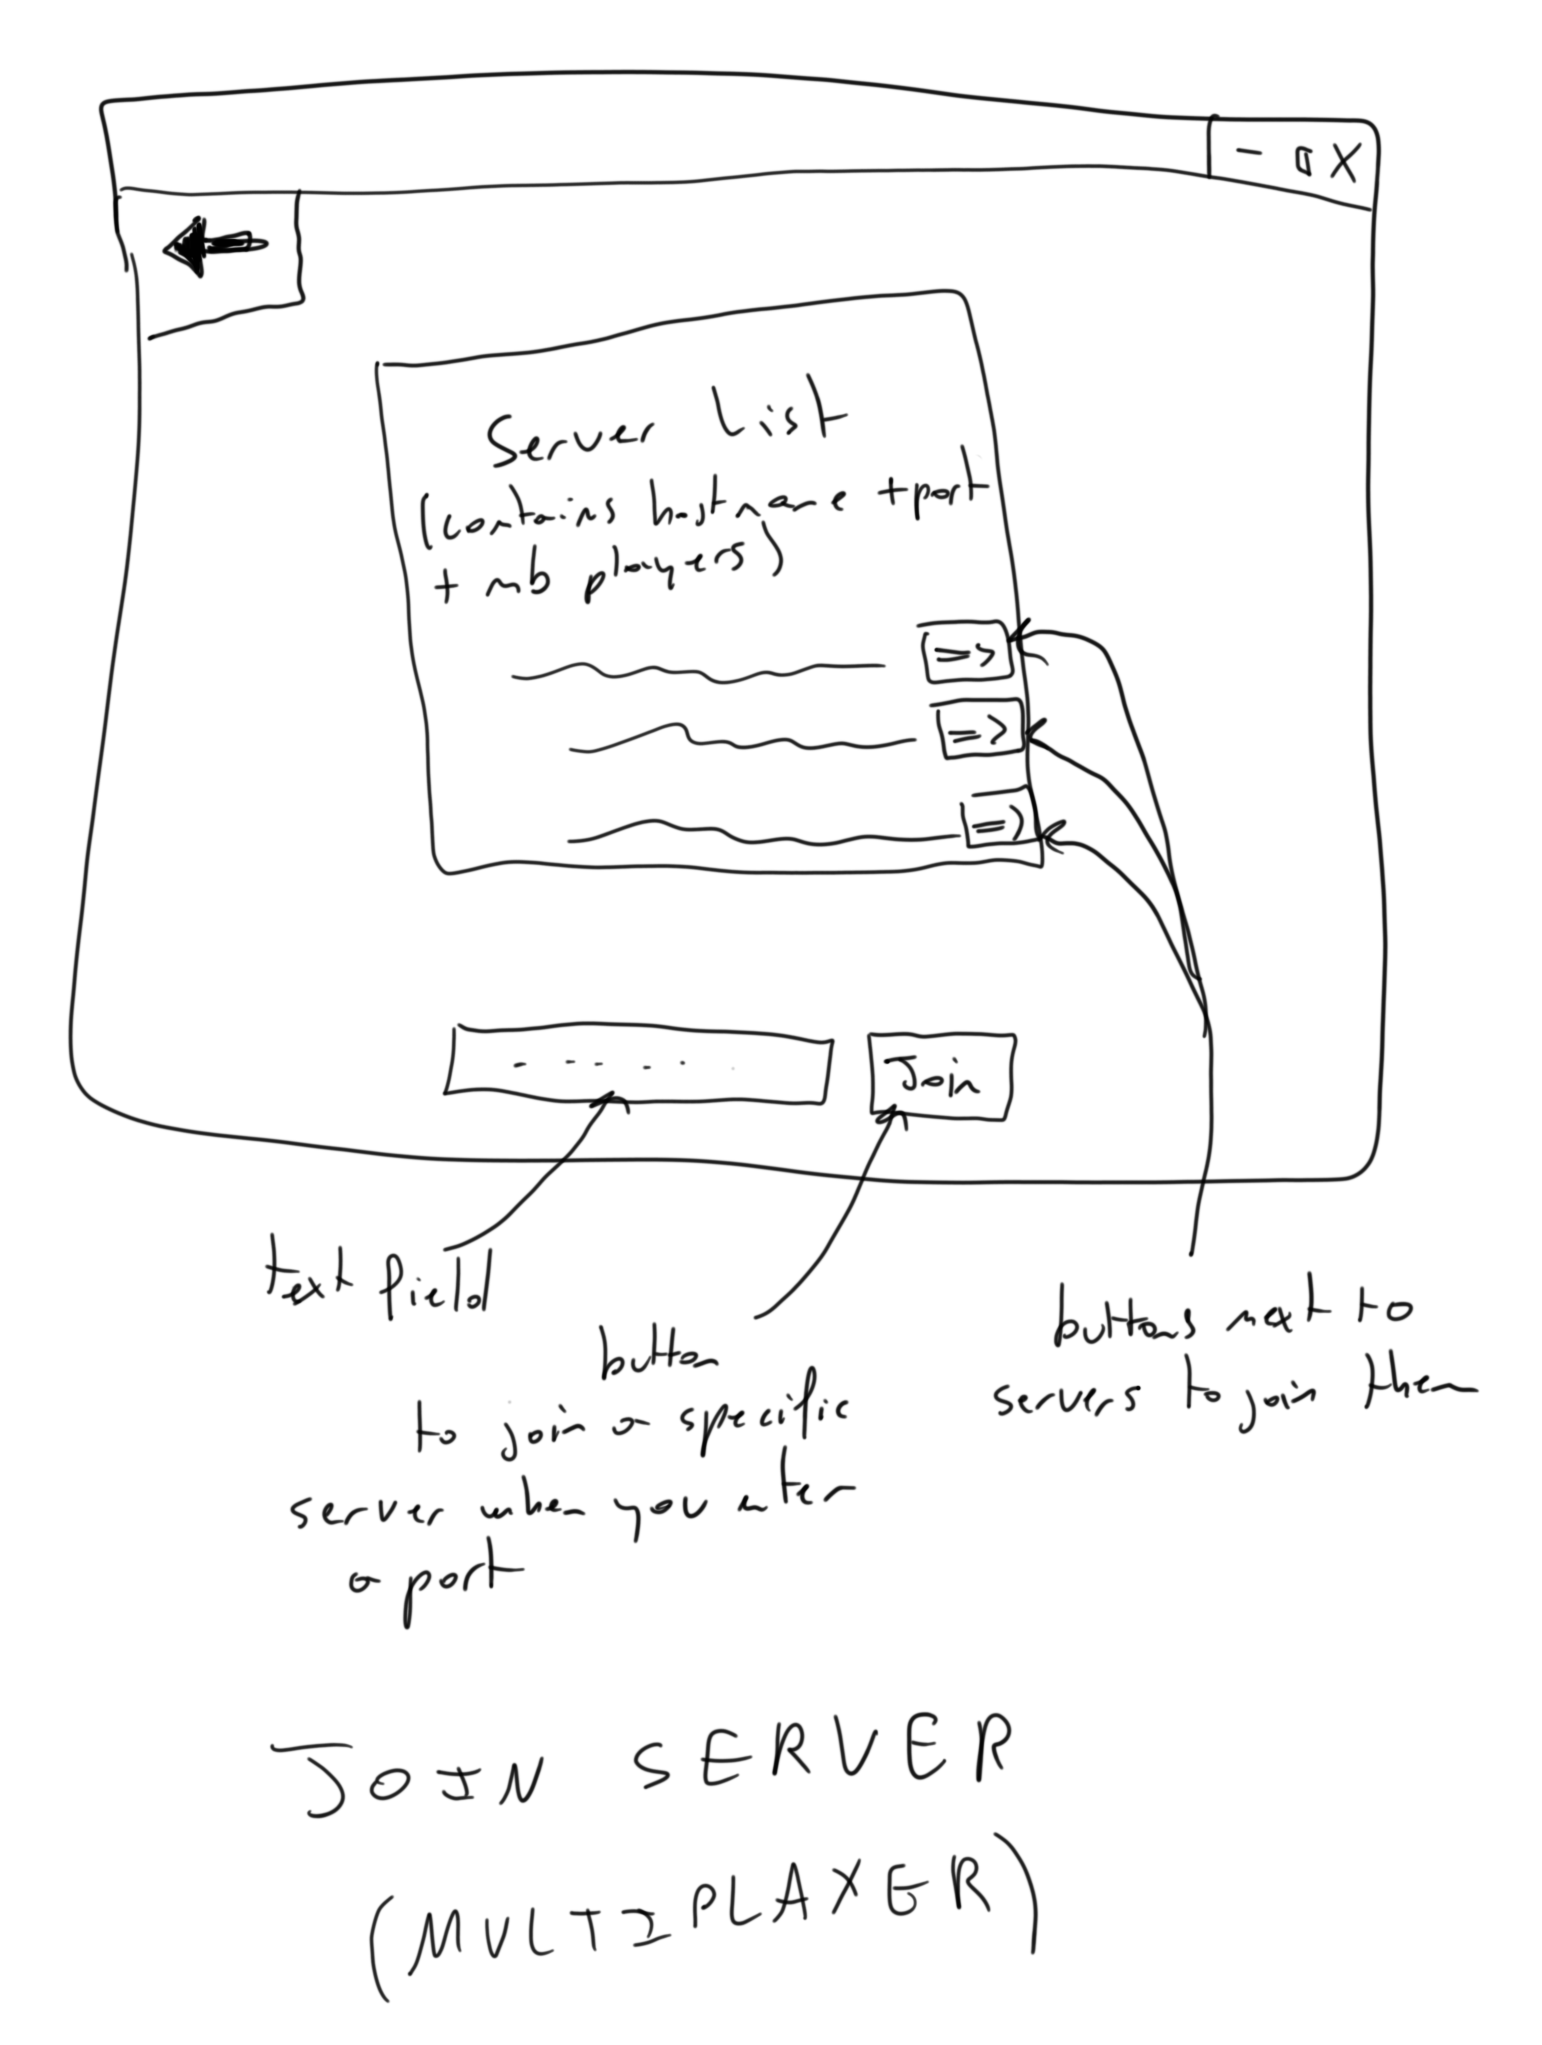
\includegraphics[width=\textwidth]{GUI_schemas/join_server_pdp.png}}
        \caption{Liste des serveurs}
        \label{fig:serv_list}
    \end{minipage}
    \hfill
    \begin{minipage}{0.53\textwidth}
        \centering
        \frame{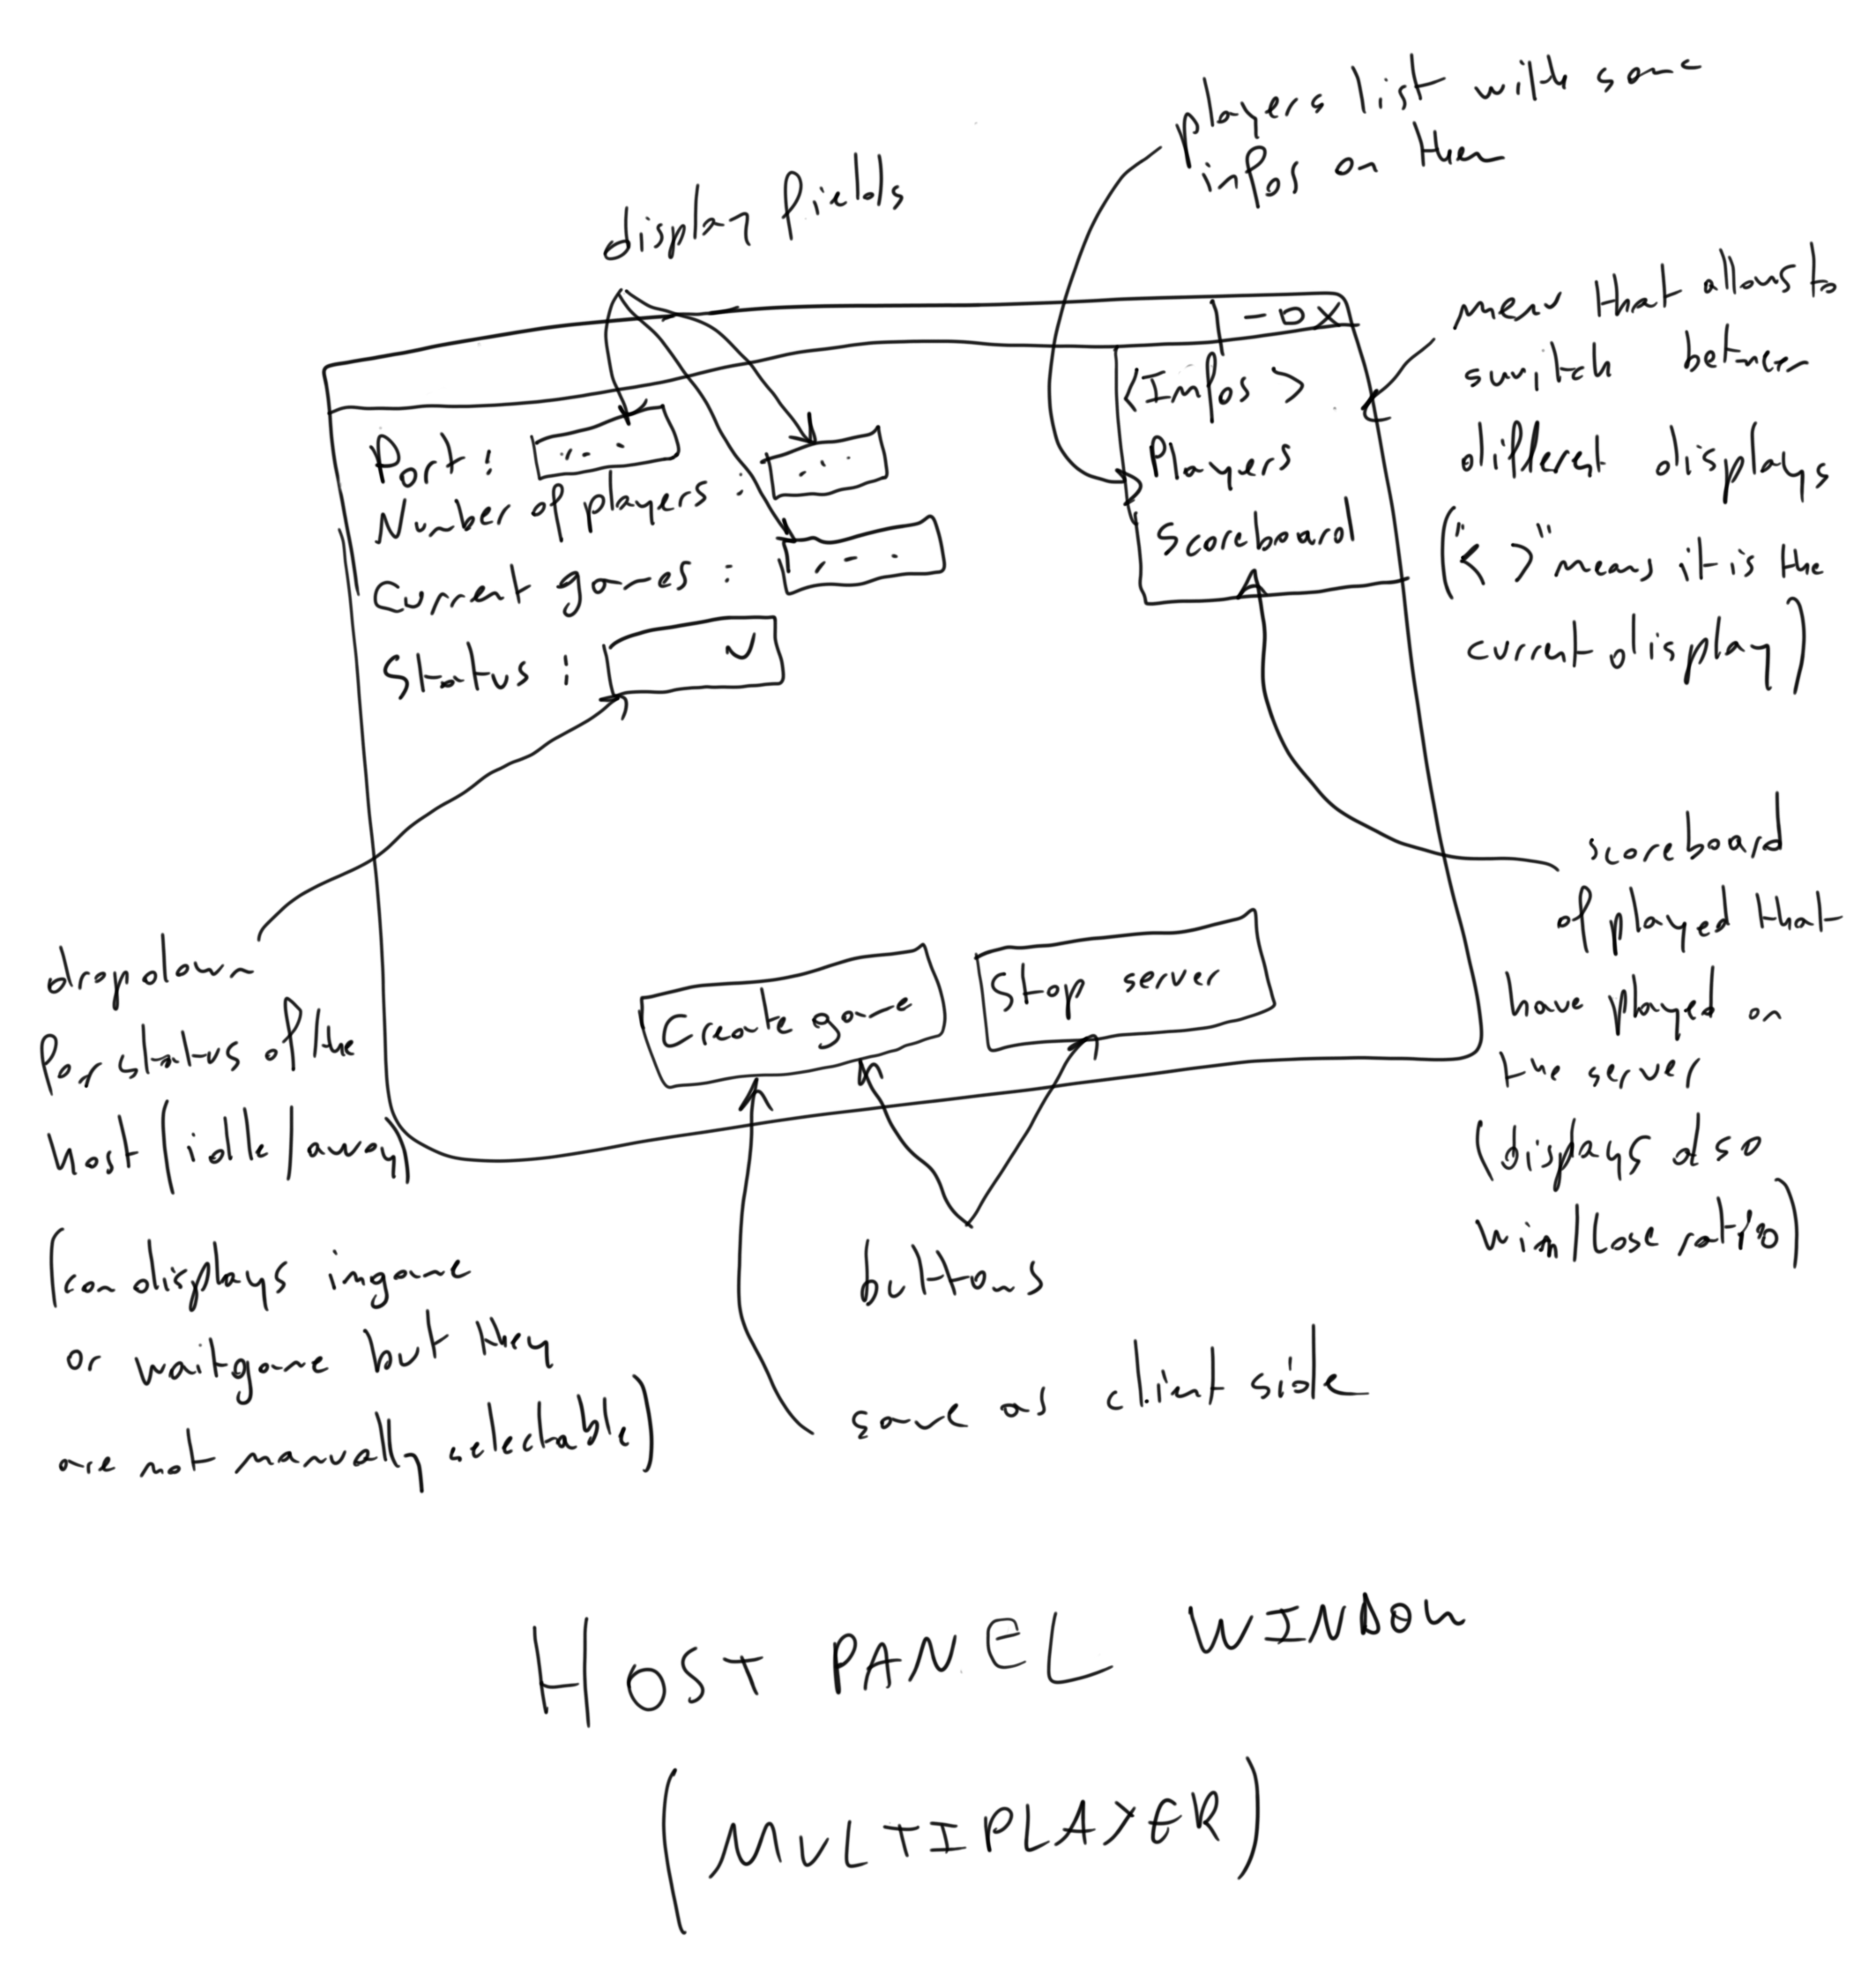
\includegraphics[width=\textwidth]{GUI_schemas/host_panel_pdp.png}}
        \caption{Menu pour le host}
        \label{fig:host_panel}
    \end{minipage}
    \end{figure}

    Pour construire l'interface avec Gtk, nous passerons par des fichiers XML. Passer par ce langage à balises simplifie la construction de l'interface en plus d'avoir une bonne intégration à Gtk par défaut. Plus précisément, les parties statiques de l'interface seront directement écrites dans les fichiers XML, tandis que les éléments dynamiques tels que les boutons ou les alertes seront codés dans les fichiers C, et feront référence à des tags de certaines balises du XML afin de pouvoir les modifier grâce au code C.
    
    De plus, Gtk offre la possibilité d'intégrer du Drag'n'Drop (pour déplacer les amazones par exemple) grâce à GtkDragSource et GtkDropTarget. On peut tester avec GtkDragSource si l'on est bien positionné sur une amazone valide (exemple : ne pas pouvoir choisir une amazone de l'autre joueur). Lorsqu'on relâche l'amazone, on fait appel à GtkDropTarget qui renverra les coordonnées (x, y) sur la fenêtre, que l'on peut ensuite passer dans une fonction de conversion pour traduire (x, y) en une case du plateau de jeu, et ainsi vérifier si cela correspond à une case valide (= si le déplacement correspond à un coup valide).
    
    \subsubsection{Intégration et CLI}
    Le module d'intégration est le pilier central de l'application. Pour garantir un code propre et éviter d'éparpiller les données dans des variables globales, nous avons regroupé tout l'état de l'application dans une structure centrale nommée \texttt{Application}.
    Cette structure contient toutes les dépendances du programme. Elle gère trois aspects essentiels : 
    \begin{itemize}
        \item \textbf{GameConfig :} Elle contient la configuration du jeu et les paramètres immuables (mode verbeux, port réseau ...) chargés au lancement ;
        \item \textbf{GameEngine* :} Un pointeur vers l'instance unique du moteur de jeu ;
        \item \textbf{Contrôle de flux :} Des drapeaux atomiques (ex: \begin{verbatim}is_running\end{verbatim}) permettant une terminaison propre et la libération des ressources via une procédure de nettoyage.
    \end{itemize}
    En parallèle, pour découpler la saisie utilisateur de l'exécution, nous utilisons une structure \texttt{UserCommand}. Elle normalise les entrées : une commande textuelle brute transformée en un type énuméré, accompagné d'arguments validés, facilitant le travail du Dispatcher.
    

    \subsection{Algorithmes utilisés} 
    \subsubsection{Réseaux}
    Bien que le projet ne nécessite pas d'algorithmes complexes en réseau, la robustesse du module repose sur trois algorithmes :
    \begin{itemize}
        \item Un algorithme de reconstruction TCP qui accumulera les données brutes dans un buffer persistant jusqu'à détecter un caractère de fin de message, puis extraira la commande complète pour traiter la fragmentation des messages ;
        \item Un algorithme de multiplexage qui utiliserait poll() pour surveiller simultanément l'activité du clavier, du serveur et des clients avec un temps d'attente nul afin d'éviter les opérations bloquantes ;
        \item Un algorithme de Routage sélectif qui parcourra la liste des clients et ne relaiera les messages qu'aux joueurs partageant le même "game id" que l'expéditeur pour éviter qu'un joueur ne reçoive les coups d'une autre partie en cours.
    \end{itemize}
    
    \subsubsection{IA}
    \paragraph{MiniMax//Alpha-Beta}
    Dû à la complexité du jeu, l'élagage standard de ces algorithmes n'est pas suffisant. Nous utiliserons alors une recherche sélective (Forward Pruning \cite{fpruning}), nous permettant d'élaguer à partir de chaque profondeur, ne gardant que les k meilleurs coups. Celle-ci se base sur l'évaluation de mobilité $(Coups_{Moi} - Coups_{Adv})$, qui est une évaluation très rapide bien que moins précise. Elle complétera les autres évaluations (Queen Distance \& King Distance, Relative Territory Heuristic).

    \paragraph{Monte Carlo Tree Search (MCTS)}
    Cet algorithme construit l'arbre de jeu de manière asymétrique et itérative. Au lieu de tout calculer, il effectue des simulations de parties pour estimer le taux de victoire des coups. En parallèle, il utilise un algorithme d'évaluation afin de sélectionner les meilleurs coups à explorer, optimisant le parcours des sous-arbres possibles.

    Parmi les algorithmes d'évaluation, nous retrouvons :
    \begin{itemize}
    \item{\textbf{Upper Confidence bounds for Trees (UCT)}} \cite{uct} :
        UCT arbitre dynamiquement entre l'exploration de coups peu visités et l'exploitation des coups prometteurs, permettant de gérer le grand facteur de branchement sans nécessiter d'évaluation experte à chaque nœud ;
    \item{\textbf{Machine Learning (ML)}} :
        Nous utiliserons un réseau de neurones (CNN) pour estimer la probabilité de victoire d'une position donnée. Ce modèle remplace la phase de simulation du MCTS : au lieu de simuler une partie, l'arbre interroge le réseau de neurones pour obtenir une évaluation directe de la feuille, gagnant ainsi du temps de calcul.
    \end{itemize}

    \subsubsection{Moteur de jeu}
        \paragraph{Génération par Ray-Casting}
        L'algorithme de génération des coups doit gérer une complexité supérieure à celle des échecs en raison de la nature composée d'un tour (Déplacement + Tir). Nous utilisons une approche de "Ray-Casting" imbriquée.
        Dans un premier temps, l'algorithme projette les déplacements possibles de l'amazone selon les 8 axes. Pour chaque case d'arrivée valide, une seconde passe de rayons est lancée pour déterminer les cibles des flèches. 

        \paragraph{Implémentation Technique}
        Pour chaque direction, le moteur charge un masque représentant un rayon théorique maximal. L'algorithme applique d'abord une intersection logique (\texttt{Rayon\&Plateau}) pour isoler les obstacles potentiels sur la trajectoire.
        Une instruction processeur de Bitscan identifie alors l'index du premier obstacle rencontré. Un second masque est ensuite généré pour éteindre toutes les cases situées au-delà de cet obstacle, ne laissant actifs que les mouvements valides.
        Une attention particulière est portée à la phase de tir. Puisque l'amazone tire après s'être déplacée, sa case de départ est libérée mais le plateau global n'est pas encore mis à jour. On applique un XOR temporaire sur le bitboard du plateau. Cette opération rend l'ancienne position libre, permettant à l'algorithme de Ray-Casting de valider un tir traversant la case que l'amazone vient de quitter.


\subsubsection{CLI}

    Le shell interactif repose sur une boucle infinie de type REPL (Read-Eval-Print Loop) qui gère les interactions homme-machine jusqu'à l'arrêt du programme.

    \paragraph{1. Saisie } L'acquisition des commandes est déléguée à la bibliothèque \texttt{GNU Readline}. Elle capture l'entrée utilisateur sous forme de chaîne brute, tout en offrant les fonctionnalités d'édition de ligne et d'historique.

    \paragraph{2. Tokenization } La chaîne brute est transmise au tokenizer qui utilise la fonction standard \texttt{strtok}. Cet algorithme découpe la chaîne en segments ("tokens") et les encapsule dans une structure intermédiaire dédiée, nommée \texttt{UserCommand}. Cette structure normalise l'entrée en isolant le type de commande (enum) et ses arguments dans un tableau fixe, facilitant leur traitement ultérieur.
    
    \paragraph{3. Exécution } L'interpréteur utilise un tableau de correspondance. Chaque entrée de ce tableau associe un mot-clé (ex: "move") à un pointeur de fonction spécifique et sa documentation. La fonction \texttt{command\_exec} parcourt cette table pour trouver une correspondance avec \texttt{args[0]}. Si un match est trouvé, la fonction du moteur de jeu associée est invoquée avec les arguments parsés.

        
    \section{Architecture}
    \subsection{Modules}
    \subsubsection{IA}    
    
    Pour la partie IA, le but était de pouvoir avoir une architecture simple à tester, simple d'utilisation, mais aussi performante et facilement modulable, en permettant l'ajout d'une IA juste à partir d'une classe et de la modification d'une liste. 
    
    Nous avons donc l'architecture présente dans la figure \ref{fig:iauml} pour répondre à ces besoins. Les paramètres donnés aux IAs seront fournis directement par le GameEngine, qui les passera au sein d'un dictionnaire (map) lors de l'initialisation, en fonction des paramètres de jeu (comme la profondeur maximale, ...). La fonction d'évaluation // la fonction de sélection feront également partie de ces paramètres, et seront assignées via init\textunderscore ai.
    
    \begin{figure}[H]
        \centering
        \makebox[\textwidth][c]{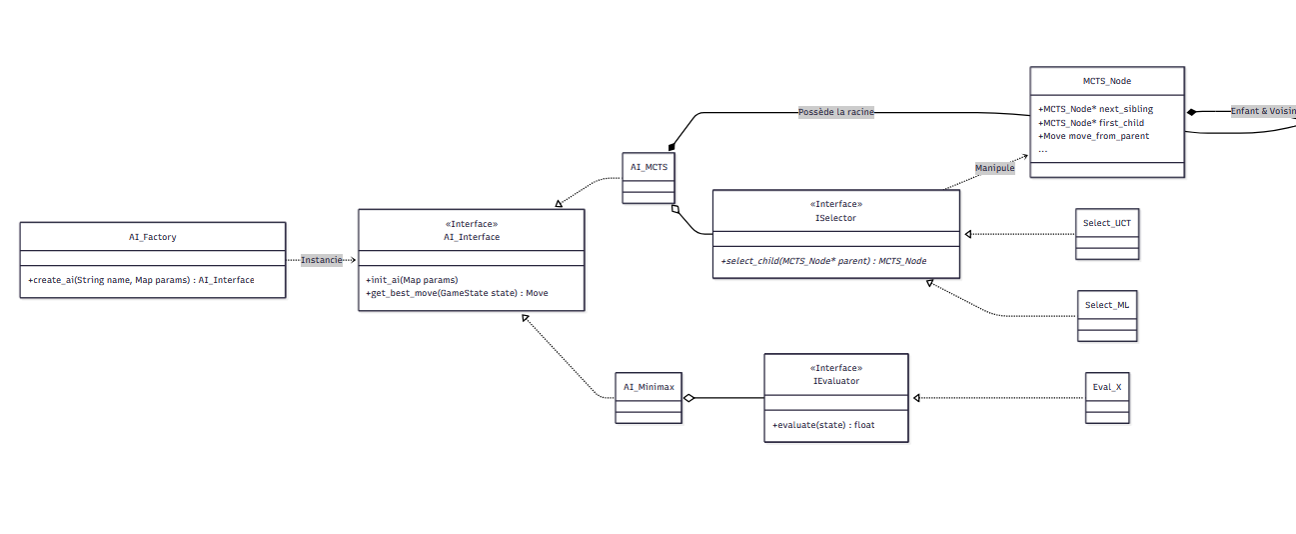
\includegraphics[width=0.75\paperwidth]{ia_uml.png}}
        \caption{IA - Diagramme UML}
        \label{fig:iauml}
    \end{figure}
    

    Comme précédemment cité (\ref{sec:iastruc}), nous avons implémenté une structure d'arbre LCRS pour MCTS, et avons utilisé des interfaces pour le polymorphisme du code.

    La dépendance entre le module IA et les autres modules ne se fera que sur le module de jeu principal, où GameEngine utilisera AI\textunderscore Factory et gardera une référence à AI\textunderscore Interface afin de pouvoir demander le meilleur coup.

    \subsubsection{Réseaux}

   
    On utilise plusieurs modules architecturaux en réseaux qui sont :
    \begin{itemize}
    \item Le premier est un pattern Façade qui n'est ni plus ni moins qu'une structure pivot contenant l'état global du réseau. Elle utilise le polymorphisme Ad-Hoc via un enum appelé "current mode" (exprimé par la cardinalité  0 ou 1 sur le diagramme). Cette structure permet au programme de décider dynamiquement d'utiliser le mode serveur et/ou client ou pas.
    Ce module à été choisit afin de centraliser la boucle d’événements et d'éviter la duplication de code. En définitive, cela permet au programme de répondre a une contrainte majeure qui est de ne jamais se bloquer, auquel cas l'interface commencerait à geler, comme en utilisant la méthode poll(). Cela garantit donc que le réseau est traité avant de mettre à jour le plateau ou de redessiner l'écran.

        \item À noter que dans la structure globale du serveur, nous maintenons un socket d'écoute (listening socket) qui ne sert qu'à accepter les connexions, tandis que les structures ConnectedClient contiennent les sockets de communication dédiés.

    \item Finalement, on utilise dans le "NetworkManager" une interface Callback. Celle-ci sert au module Réseaux à ne pas dépendre des règles du jeu pour acheminer l'information au contrôleur, qui sera alors le seul à pouvoir traiter l'information reçue. De plus, cela permet d’éviter de créer une dépendance circulaire en devant appeler le jeu pour vérifier les coups. Le NetworkManager dit simplement "j'ai reçu tel packet et ce sera au contrôleur de décider quoi faire de l’événement que décrit ce packet".
    \end{itemize}

     \begin{figure}[H]
        \centering
        \makebox[\textwidth][c]{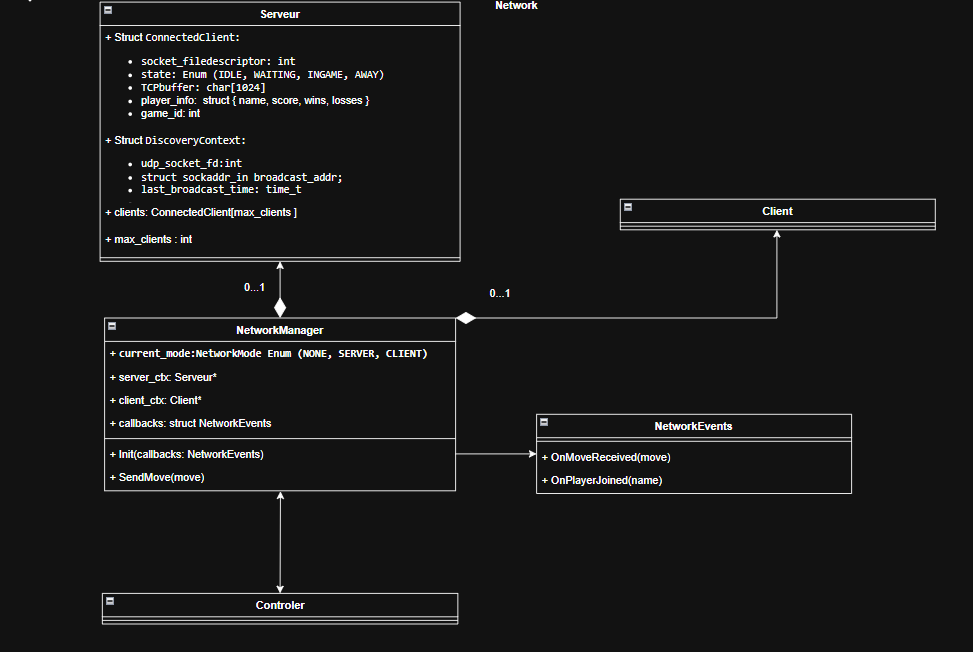
\includegraphics[width=0.65\paperwidth]{umlReseaux.png}}
        \caption{Réseaux - Diagramme UML}
        \label{fig:rsuml}
    \end{figure}
    
    
    
    \subsection{Dépendances}
    
    Pour ce qui est des dépendances de l'architecture réseaux, on utilise essentiellement la bibliothèque native / système (POSIX) avec la Berkeley Sockets API, et la librairie readline comme demandée dans le sujet.
    
    Pour l'IA, il y a une dépendance des Nodes du MCTS sur les Moves et avec les Bitboards.
    
    \section{Spécifications} 
    \subsection{Réseaux}
    \subsubsection{Découverte de service}
    F38. Le client doit pouvoir voir automatiquement les serveurs de jeu actifs sur le réseau local via un broadcast, éliminant le besoin de connaître l'adresse IP cible à l'avance.

    Prérequis: GUI (F28) et CLI (F15), Support du protocole UDP et configuration du socket avec l'option "SO BROADCAST".
      
    Architecture découplée : Le serveur utilise une structure (DiscoveryContext) pour émettre périodiquement des paquets (contenant : Nom du serveur, Port TCP, Statut) sans bloquer le jeu. Le client écoute sur un port (ex: 8081). 
    
    Signatures des fonctions :
    
    Serveur : \begin{verbatim}void broadcast_presence(int udp_socket, int tcp_port, const char* server_name);\end{verbatim}
    
    Client : \begin{verbatim}server_list_t* client_scan_for_servers(int timeout_ms);\end{verbatim}
    
    Validation : Lancer une instance serveur sur une machine A. Sur une machine B (sans configurer préalablement), lancer la commande server list et vérifier que l'IP et le nom de la machine A apparaissent immédiatement. Vérifier avec Wireshark que les paquets UDP sont bien envoyés à l'adresse de diffusion 255.255.255.255. Vérifier également que l'affichage GUI fonctionne bien, et que les commandes CLI sont bien existantes.
    
    \section{Transparence IA}

    Durant le projet, l'IA (Gemini 3.0) a été utilisée à la manière d'un moteur de recherche, et également à but informatif. Des exemples d'utilisations sont :
    \begin{itemize}
        \item Résumé d'informations contenues dans des papiers de recherche ;
        \item Explication de concepts clés et vulgarisation scientifique (exemple : explication calculs Queen Distance \& King Distance, ...) ;
        \item Vérification de logique directe d'architecture ;
        \item Exemples réduits de codes possibles, par rapport à d'autres scénario (exemple : pseudo-code MCTS pour comprendre le fonctionnement de son architecture) ;
        \item Aide à la mise en page du rapport (certaines commandes Latex).
    \end{itemize}
    
    % --- Bibliographie ---
    \newpage
    \markboth{}{} 
    
    % 1. On l'ajoute au sommaire en tant que "part"
    \addcontentsline{toc}{part}{Références bibliographiques} 
    
    % 2. On crée le titre de la page (centré et gras comme une partie)
    \begin{flushleft}
        \huge\bfseries Références bibliographiques
    \end{flushleft}
    \vspace{1.5cm} % Espace entre le titre et la liste

    % 3. On affiche la liste
    \nocite{*} 
    \printbibliography[heading=none]

    \appendix



\end{document}